% Docker Meetup at MfN, 24 April 2018
% Running wikis at the Museum with Docker - past, present and future
% Alvaro Ortiz-Troncoso
% 
% Template:
% see https://en.wikibooks.org/wiki/LaTeX/Presentations

\documentclass[13pt]{beamer}
\usepackage[utf8]{inputenc}
\usepackage{graphicx}
\usepackage{xcolor}

\definecolor{mfn_green}{HTML}{A1BF23}
\setbeamercolor{title}{fg=black}
\setbeamerfont{title}{family=\sffamily,series=\bf}
\setbeamercolor{frametitle}{fg=black}
\setbeamerfont{subtitle}{family=\sffamily,shape=\itshape}
\beamertemplatenavigationsymbolsempty
\setbeamertemplate{footline}[page number]
\setbeamertemplate{itemize item}{\color{mfn_green}$\blacktriangleright$}
\setbeamertemplate{caption}{\tiny \insertcaption}
\setbeamersize{text margin left=5mm,text margin right=5mm}
%Running wikis at the Museum with Docker: past, present and future The Museum outputs exhibitions, science papers, conferences, and so much more. None of this would be %possible without cooperation between researchers, designers, organizers and of course admins and developers. Wikis were introduced at the Museum in 2014 as an %experiment to improve  cooperation within project teams. I'll talk about how Docker solves many of the problems of running a bunch of wikis on a string, and also %about pending questions we are currently trying to answer.
%I am a computer scientist and joined the Museum in 2014. I have worked at the Technische Universität Berlin and at Waag Technology & Society in Amsterdam.

\title
{Running wikis at the Museum with Docker}
\subtitle{past, present and future}
\author
{Alvaro Ortiz-Troncoso}
\date
{Docker Meetup at Museum für Naturkunde Berlin, 2018}
\subject{Computer Science}

\begin{document}

% 1. Titelseite
{
  \logo{
\includegraphics[height=1cm]{mfn_logo_klein.png}\vspace{220pt}}
  \frame{\titlepage}
}

% 2. Das Museum
\begin{frame}
  \frametitle{Das Museum / \textcolor{mfn_green}{The Museum}}
  \begin{figure}
    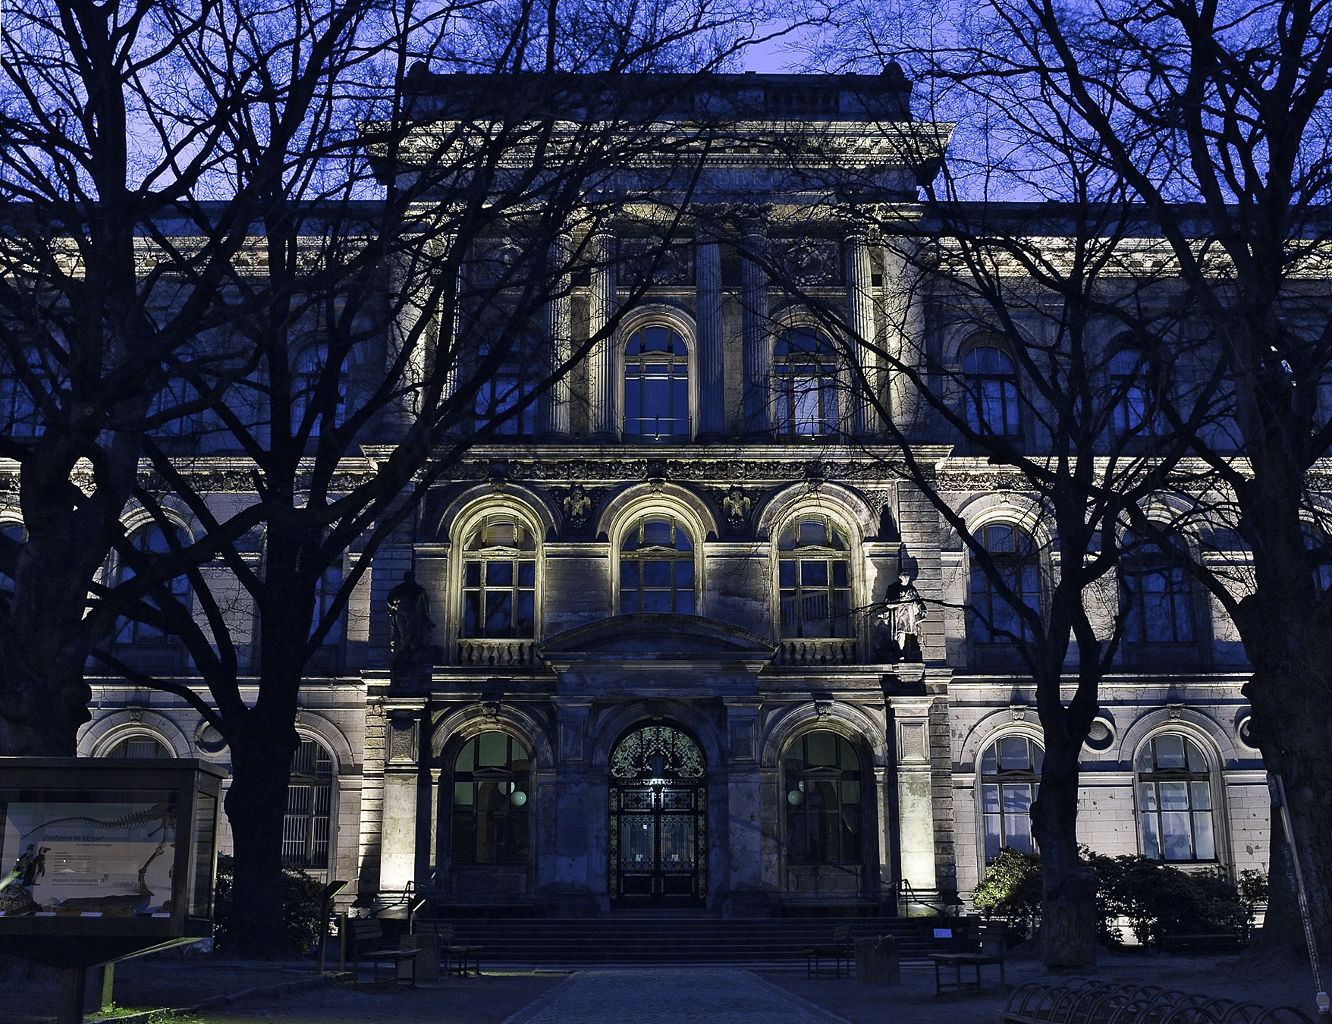
\includegraphics[height=70mm]{Gebaeude_Nacht.jpg}
    \caption{\textcopyright Antje Dittmann, Museum für Naturkunde Berlin, 2009. CC-by-sa}
  \end{figure}
\end{frame}

% 3. Ausstellung
\begin{frame}
  \frametitle{Die Ausstellung / \textcolor{mfn_green}{The exhibition}}
  \begin{figure}
  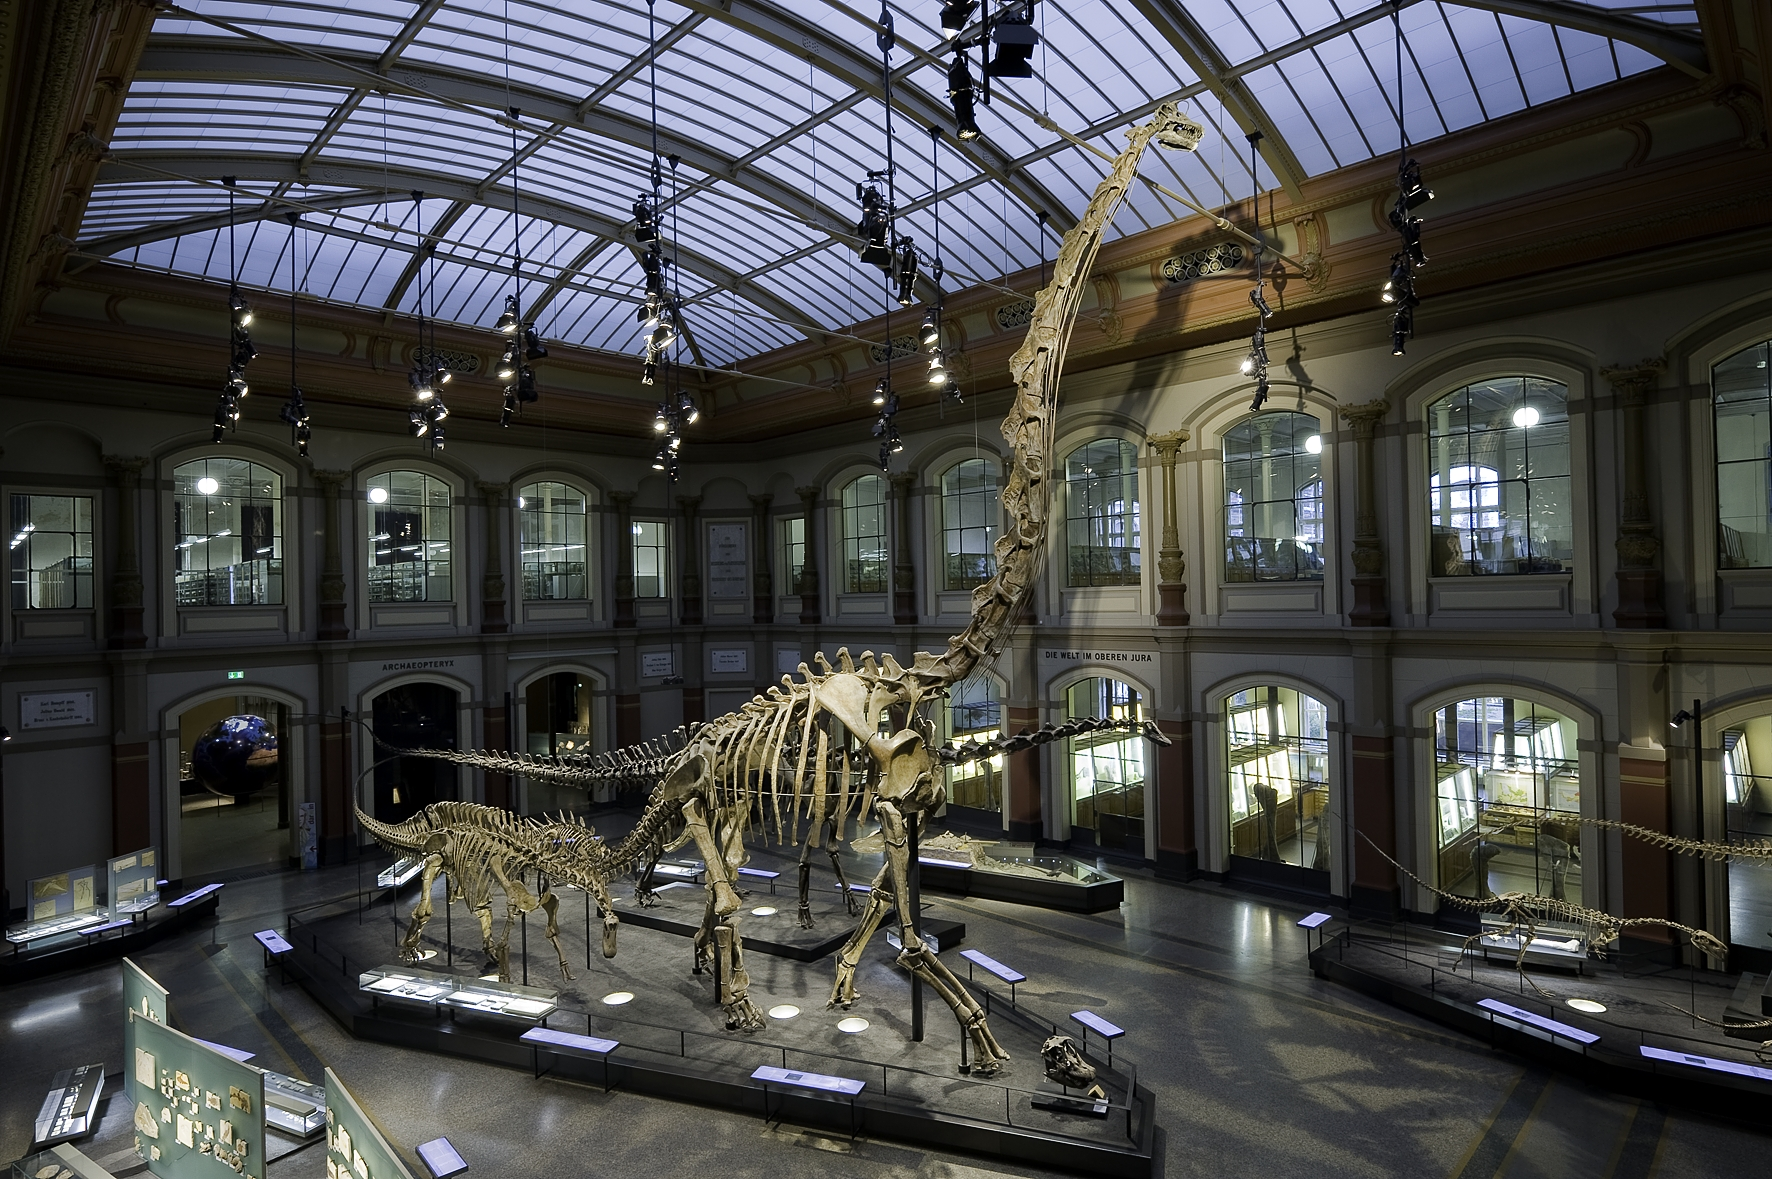
\includegraphics[height=70mm]{Brachiosaurus_02_15cm.jpg}
  \caption{\textcopyright Antje Dittmann, Museum für Naturkunde Berlin, 2009. CC-by-sa}
  \end{figure}
\end{frame}

% 4. Numbers
\begin{frame}
  \frametitle{ Einige Zahlen / \textcolor{mfn_green}{Some numbers}}

  \begin{itemize}
  \item{Personal: 289, Studenten: 209}
  \item{Publikationen: 222 / Jahr (2016)}
  \item{Aktuell erforschen 51 Projekte die Sammlung}
  \end{itemize}
  
  \begin{itemize}
  \item{\textcolor{mfn_green}{Staff: 289, Students: 209}}
  \item{\textcolor{mfn_green}{Publications 222 / year (2016)}}
  \item{\textcolor{mfn_green}{Currently 51 projects are researching the collection}}
  \end{itemize}
  \bigskip
  \tiny{Unsere Wissenschaft / Our Science, DOI: 10.7479/3dwq-8a7g}
\end{frame}


% 5. Forschungsprojekte
\begin{frame}
  \frametitle{Forschungsprojekte / \textcolor{mfn_green}{Research projects}}
  \begin{figure}
  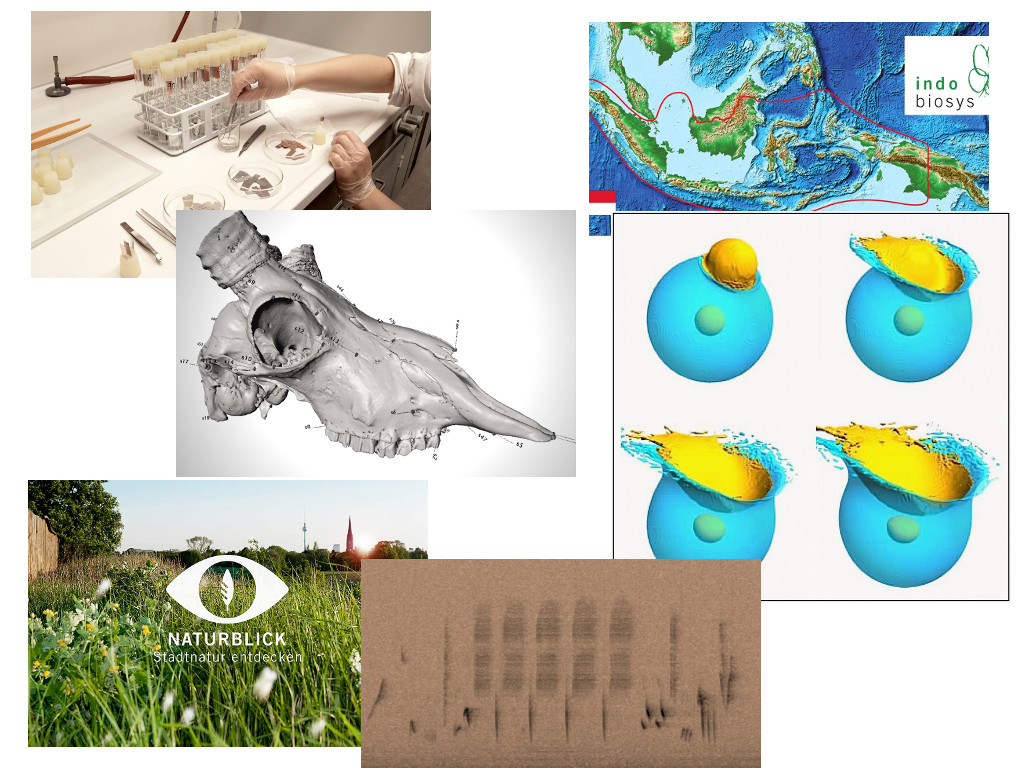
\includegraphics[height=70mm]{Forschung.jpg}
  \end{figure}
\end{frame}

% 6. Was macht ein Projekt aus?
{
\setbeamercolor{background canvas}{bg=mfn_green}
\setbeamercolor{frametitle}{fg=black}
\begin{frame}
  \frametitle{Was macht ein Projekt aus? \\ \textcolor{white}{What does it take to launch a project?}}
  \begin{figure}
  \includegraphics[height=70mm,trim=4 4 4 4,clip]{Projekt.png}
  \end{figure}
\end{frame}
}

% 7. Kooperation
\begin{frame}
  \frametitle{Kooperation / \textcolor{mfn_green}{Cooperation}}

  \begin{itemize}
  \item{Gemeinsames Verständnis der Projektziele}
  \item{Innerhalb des Zeitrahmens zum Ergebnis kommen}
  \item{Den Kostenrahmen nicht überschreiten - Effizient arbeiten}
  \end{itemize}
  
  \begin{itemize}
  \item{\textcolor{mfn_green}{Common understanding of project goals}}
  \item{\textcolor{mfn_green}{Deliver on time}}
  \item{\textcolor{mfn_green}{Be efficient to finish within budget}}
  \end{itemize}
\end{frame}

%%%%%%%%%%%%%%%
%
% The past
%
%%%%%%%%%%%%%%%

% 8. In der Vergangenheit
\begin{frame}
  \frametitle{In der Vergangenheit / \textcolor{mfn_green}{In the past}}
  \begin{figure}
    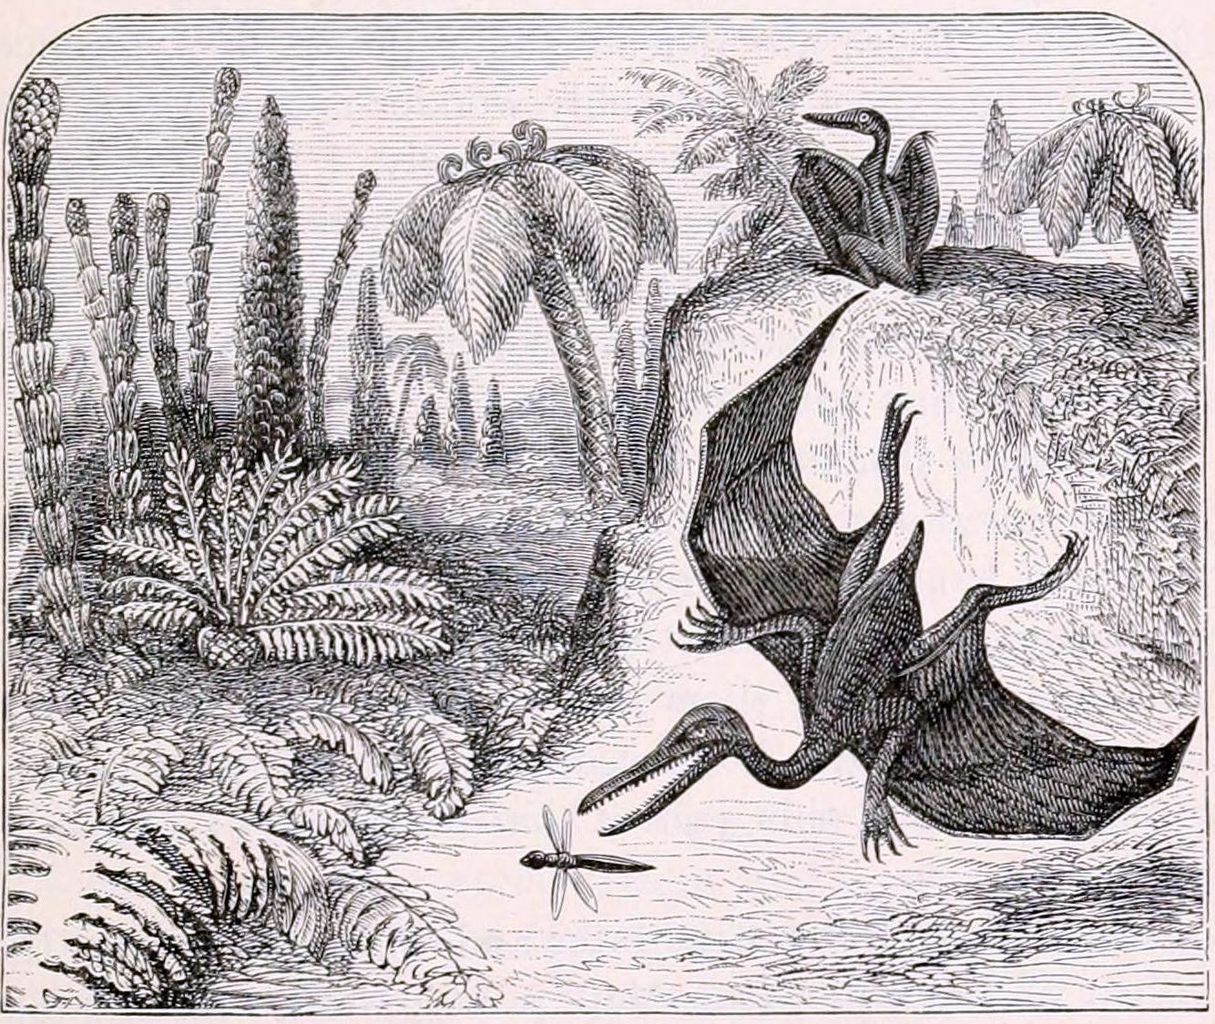
\includegraphics[height=70mm]{Ideal_Landscape_of_a_Prehistoric_Age.jpg}
    \caption{Quackenbos, J.D., 1886. \textit{Illustrated School History of the World}. D. Appleton.}
  \end{figure}
\end{frame}

% 9. Word .doc Hölle
{
\setbeamercolor{background canvas}{bg=mfn_green}
\setbeamercolor{frametitle}{fg=black}
\begin{frame}
  \frametitle{Word\textsuperscript{\tiny\textregistered} .doc Hölle /
    \textcolor{white}{Word\textsuperscript{\tiny\textregistered} .doc hell}}
  \begin{figure}
  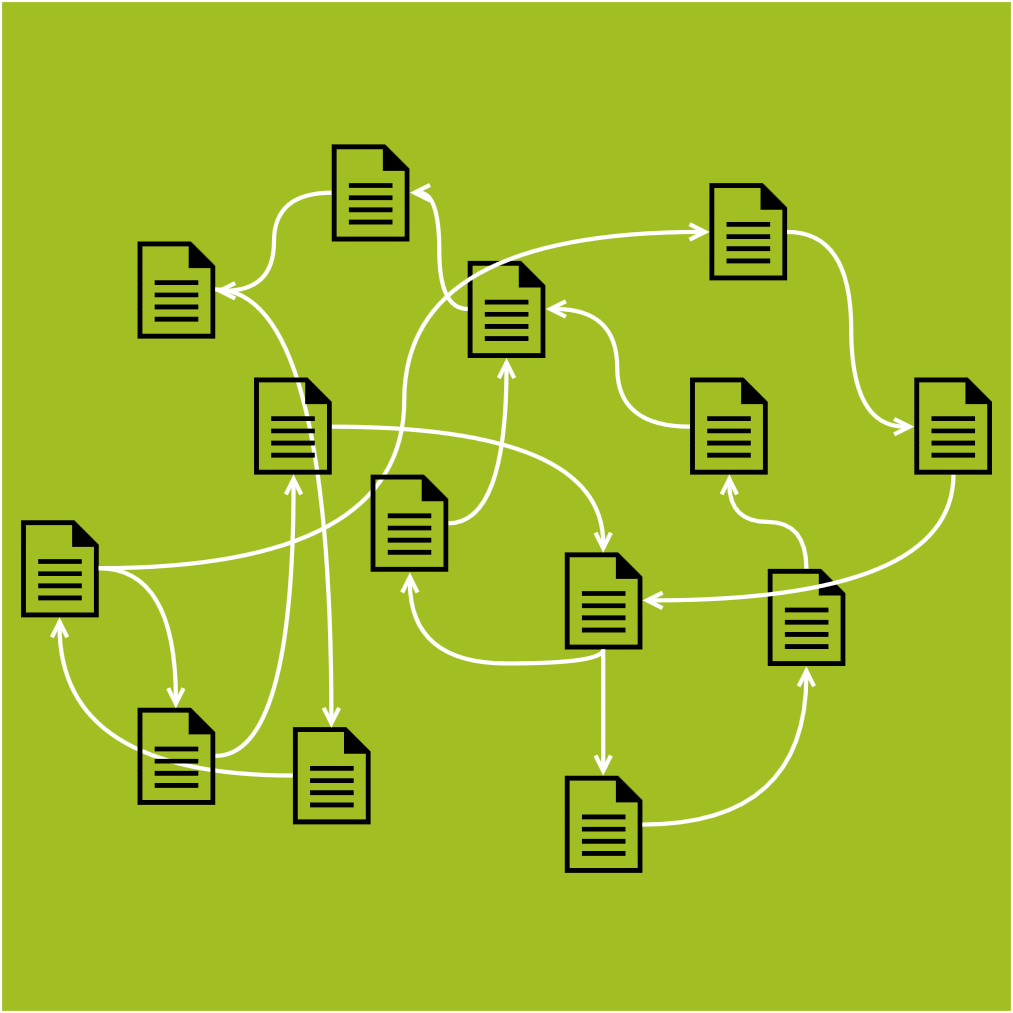
\includegraphics[height=70mm,trim=4 4 4 4,clip]{Docs.png}
  \end{figure}
\end{frame}
}

% 10. Nichts gegen Word aber...
\begin{frame}
  \frametitle{Nichts gegen Word\textsuperscript{\tiny\textregistered} aber... \\
    \textcolor{mfn_green}{Absolutely nothing against Word\textsuperscript{\tiny\textregistered}, however, ...}}
  \begin{itemize}
  \item{Keine Versionierung: wer hat die Endfassung?}
  \item{Kein Dokumentverlauf: wer hat was geschrieben?}
  \item{Proprietäre Software: Anbieterabhängigkeit}
  \end{itemize}
  
  \begin{itemize}
  \item{\textcolor{mfn_green}{No versioning: who has the final version}}
  \item{\textcolor{mfn_green}{No document history: who wrote what?}}
  \item{\textcolor{mfn_green}{Proprietary software: vendor lock-in}}
  \end{itemize}
\end{frame}

%%%%%%%%%%%%%%
%
% The present
%
%%%%%%%%%%%%%%

% 11 Beispiel Panda-Wiki
\begin{frame}
  \frametitle{Konkretes Beispiel: das Panda-Wiki\\\textcolor{mfn_green}{A specific example: the Panda wiki}}
  \begin{figure}
    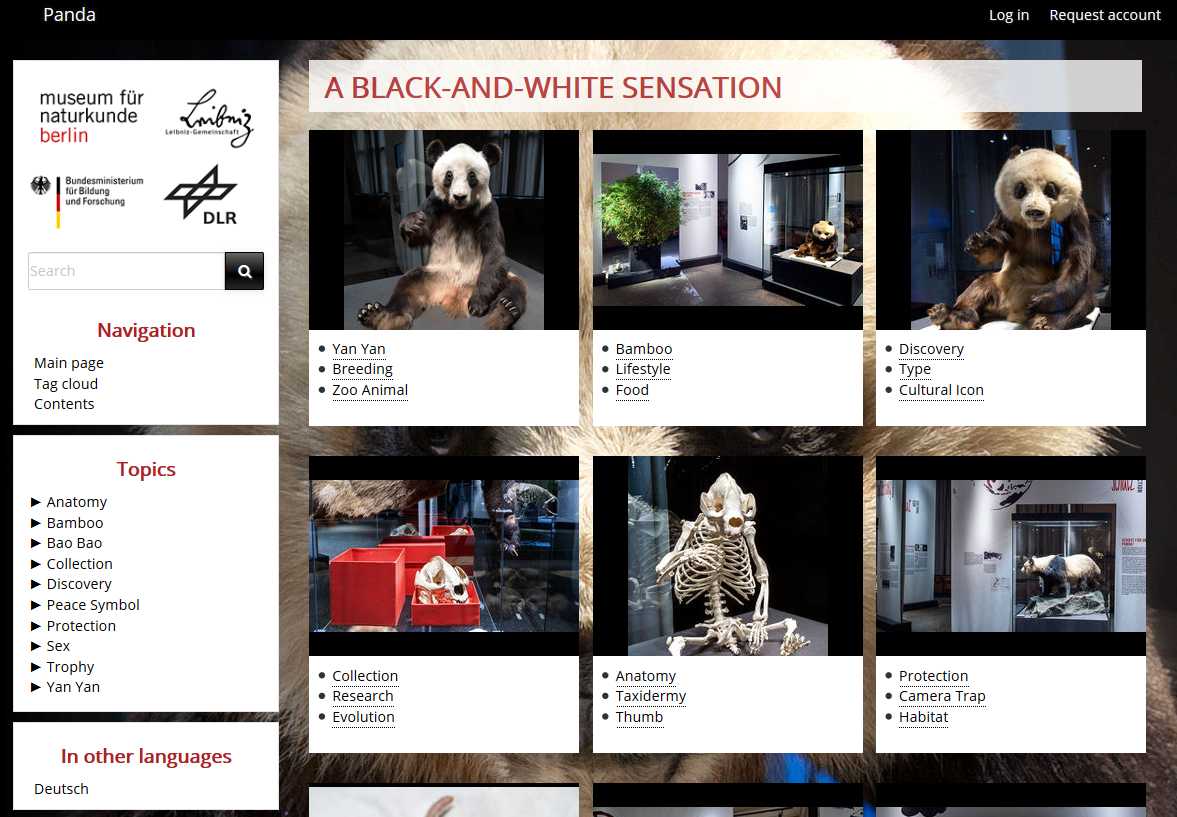
\includegraphics[height=60mm]{panda.png}
    \caption{http://biowikifarm.net/v-mfn/panda}
  \end{figure}
\end{frame}

% 12. Wikis am Museum
\begin{frame}
  \frametitle{Wikis am Museum / \textcolor{mfn_green}{Wikis at the Museum}}

  \begin{itemize}
  \item{Forschungsprojekte können ein Wiki nutzen, sofern sie es wünschen}
  \item{Wikis sind standardmäßig privat, können aber zum Teil oder im Ganzen geöffnet werden}
  \item{Wikis sind semantisch: sie können sowohl mit Freiformtexten als auch mit strukturierten Daten umgehen}
  \end{itemize}
  
  \begin{itemize}
  \item{\textcolor{mfn_green}{Research projects may use a wiki if they wish to do so}}
  \item{\textcolor{mfn_green}{Wikis are private by default, but may be made public in part or in whole}}
  \item{\textcolor{mfn_green}{Wikis are semantic, so can be used with plain texts as well as with structured data}}
  \end{itemize}
\end{frame}

% 13. Die derzeitige Praxis
\begin{frame}
  \frametitle{Die derzeitige Praxis / \textcolor{mfn_green}{The present}}
  \begin{figure}
    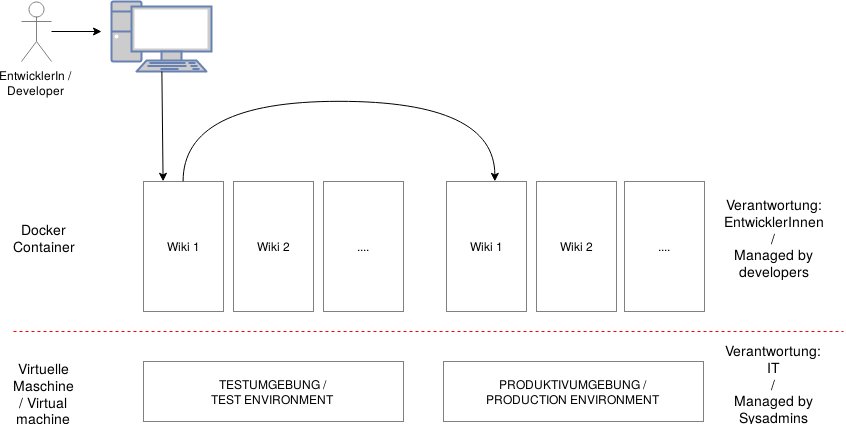
\includegraphics[width=110mm]{docker_wikis.png}
  \end{figure}
\end{frame}

% 14. Rollout UML
\begin{frame}
  \frametitle{Rolloutprozess / \textcolor{mfn_green}{Rollout process}}

  \begin{figure}
    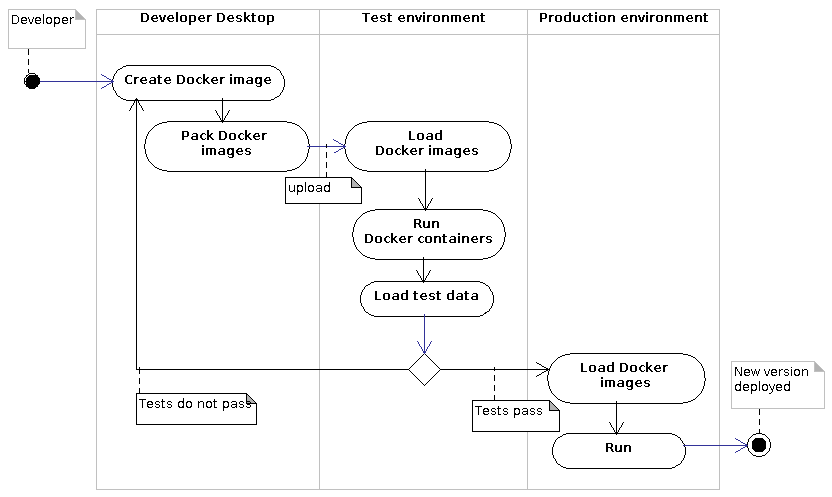
\includegraphics[width=\textwidth]{deploy_wiki_uml.png}
  \end{figure}

\end{frame}

%%%%%%%%%%%%%%
%
% The future
%
%%%%%%%%%%%%%%

% 15. Blick in die Zukunft
\begin{frame}
  \frametitle{Blick in die Zukunft \\ \textcolor{mfn_green}{The shape of things to come}}
  \begin{figure}
    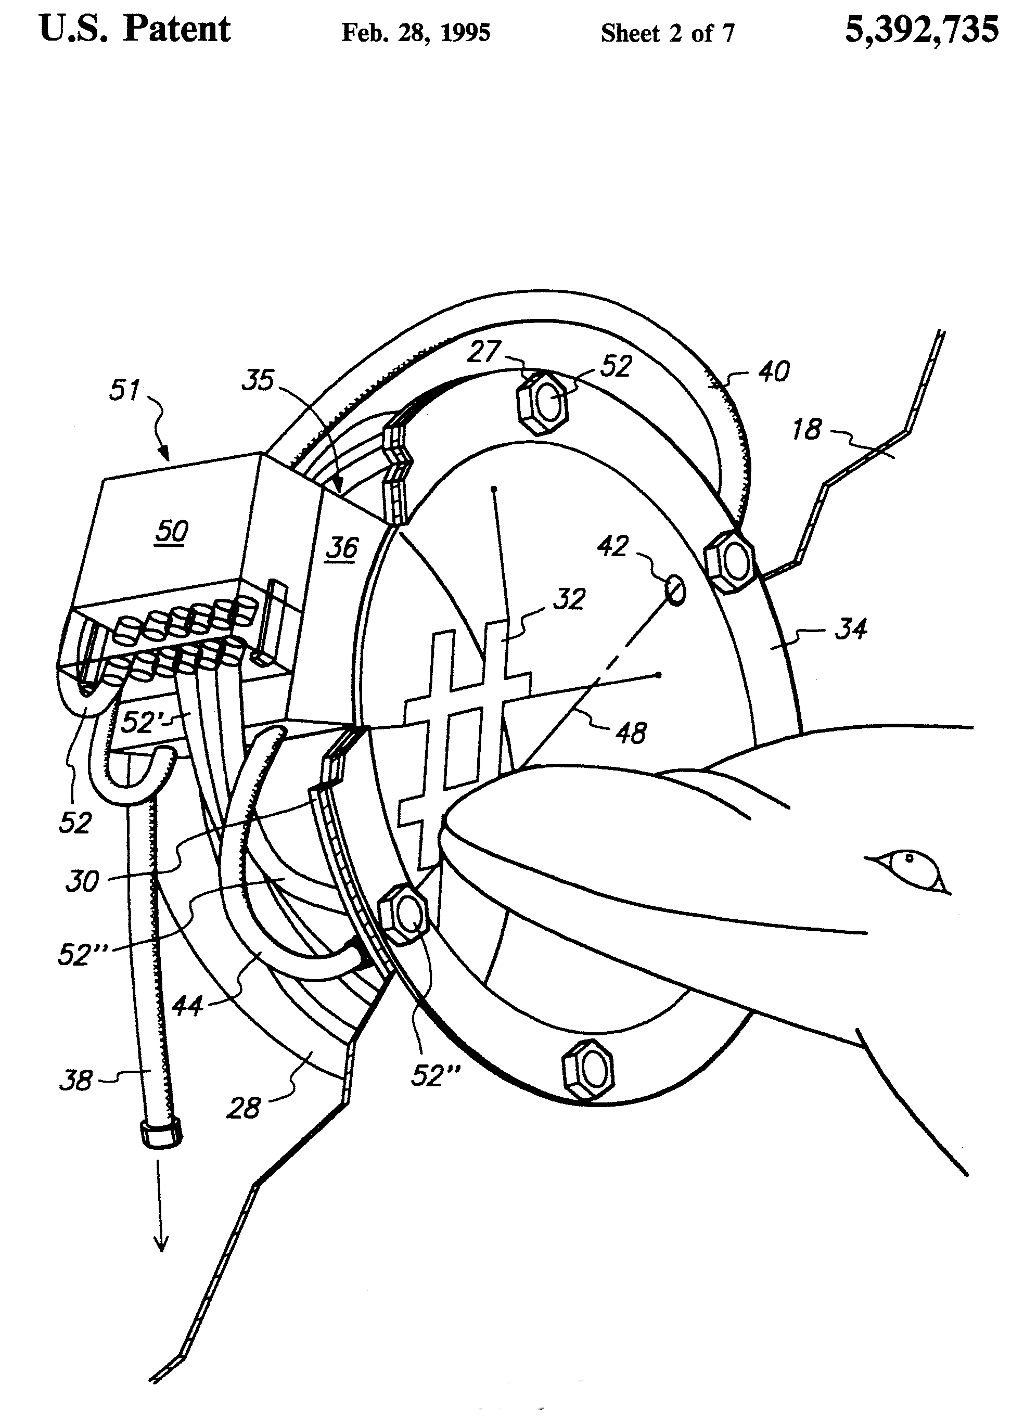
\includegraphics[height=60mm]{marine_mammal_communication.png}
    \caption{Xitco Jr, M.J. et al, 1995. \textit{Marine mammal communication device}. U.S. Patent 5,392,735.}
  \end{figure}
\end{frame}

% 16. Problemzone
\begin{frame}
  \frametitle{Problemzone / \textcolor{mfn_green}{Problem zone}}
  \begin{figure}
    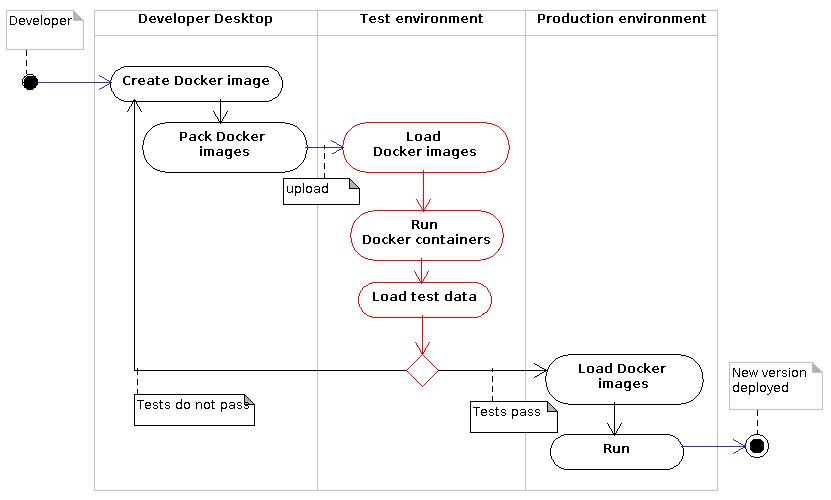
\includegraphics[width=\textwidth]{docker_wikis_problem_uml.png}
  \end{figure}
\end{frame}

% 17. Lösungsansatz
\begin{frame}
  \frametitle{Lösungsansatz / \textcolor{mfn_green}{Planed solution}}
  \begin{figure}
    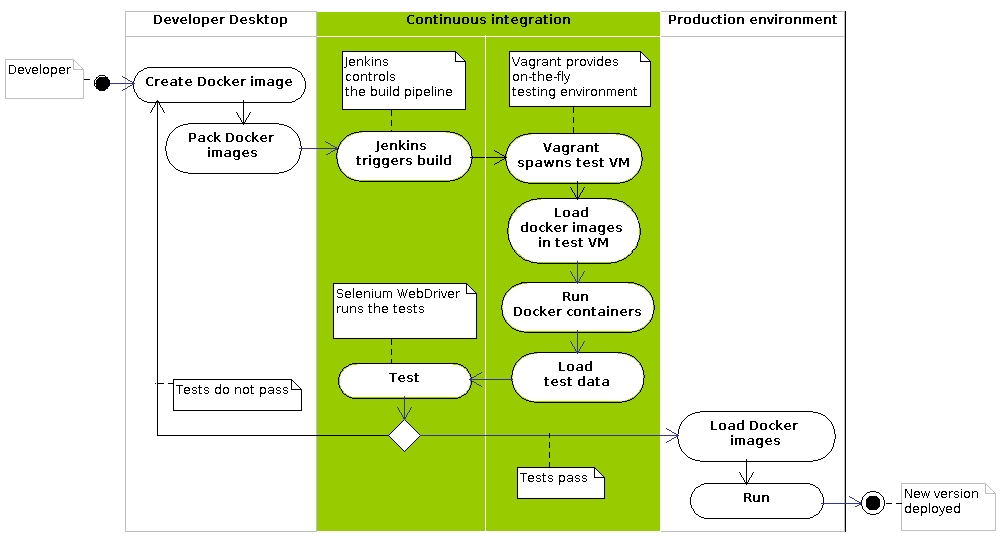
\includegraphics[width=\textwidth]{docker_wikis_integration.png}
  \end{figure}
\end{frame}

% 18. Kontaktdaten
\begin{frame}
  \frametitle{Kontaktdaten / \textcolor{mfn_green}{Contact information}}
  \begin{center}
    Alvaro Ortiz-Troncoso \\
    \medskip
    Email: Alvaro.OrtizTroncoso@mfn.berlin \\    
    \medskip
    Web: https://github.com/MfN-Berlin
  \end{center}
\end{frame}

\end{document}


